\section{系统安装调试}
本章详细介绍了基于CH32微控制器的气垫船控制系统的安装与调试过程。安装调试是确保系统可靠运行的关键环节，主要包括硬件模型的安装、各功能模块的单独调试以及系统的整体联调。
% \subsection{硬件模型安装}
\subsection{主控模块 PCB 安装}
硬件安装中，采用SMD贴片工艺焊接CH32V307微控制器，控制引脚对齐与焊接温度以确保连接可靠。电源部分通过稳压电路提供3.3V供电，并在关键节点配置去耦电容以滤除噪声。时钟电路使用8MHz晶振与22pF匹配电容，通过优化布局保障时钟稳定。最后安装标准SWD调试接口，采用2.54mm排针引出，便于连接调试工具进行程序下载与在线调试，如图\ref{zhu-kong}所示。
\begin{figure}[h]
    \centering
    \subfigure[主控模块 PCB 正面]{
    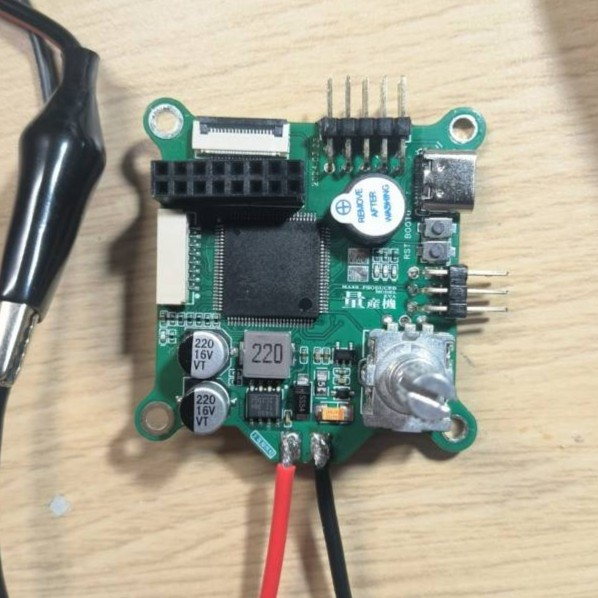
\includegraphics[scale=0.4]{./pic/chapter05/zhu-kong-zheng.jpg} 
    }
    \quad
    \subfigure[主控模块 PCB 反面]{
    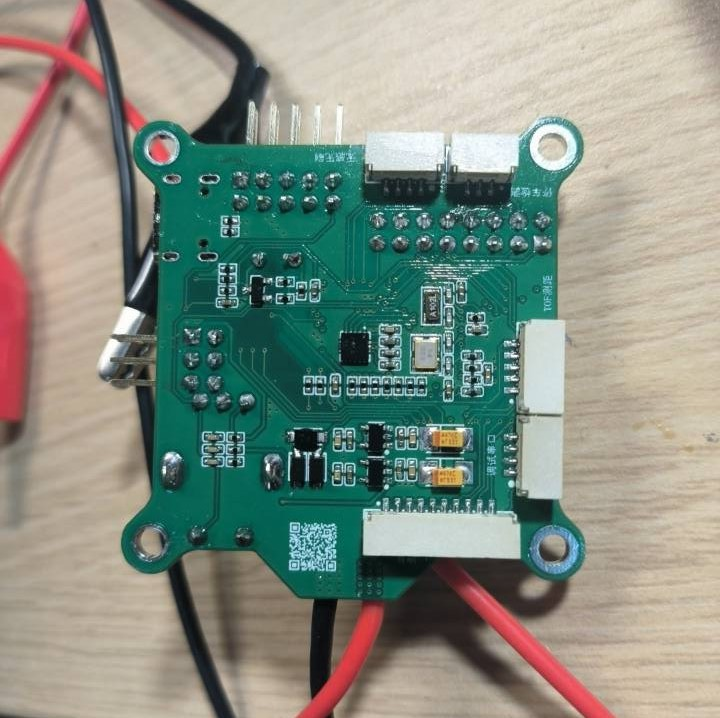
\includegraphics[scale=0.33]{./pic/chapter05/zhu-kong-fan.jpg}  
    }
    \caption{主控模块 PCB}
    \label{zhu-kong}
    \end{figure}
    
\subsection{有刷驱动 PCB 安装}
驱动系统采用四路独立H桥电路驱动有刷电机，每路均配备上下桥臂MOS管与专用栅极驱动芯片以实现精准的开关控制。电源端采用电解电容与陶瓷电容组合滤波，有效抑制电压波动；输出端配置自恢复保险丝与TVS二极管，提供过流与反电动势保护。PCB布局优先保证大电流路径最短，采用星型单点接地与信号包地设计以降低干扰。散热方面通过厚铜层与铝合金基板配合导热硅胶垫确保散热效率，功率端子选用带锁紧机制的接口防止松动，并通过光耦隔离控制信号与功率电路，提升系统可靠性，如图\ref{you-shua}所示。
\begin{figure}[htbp]
    \centering
    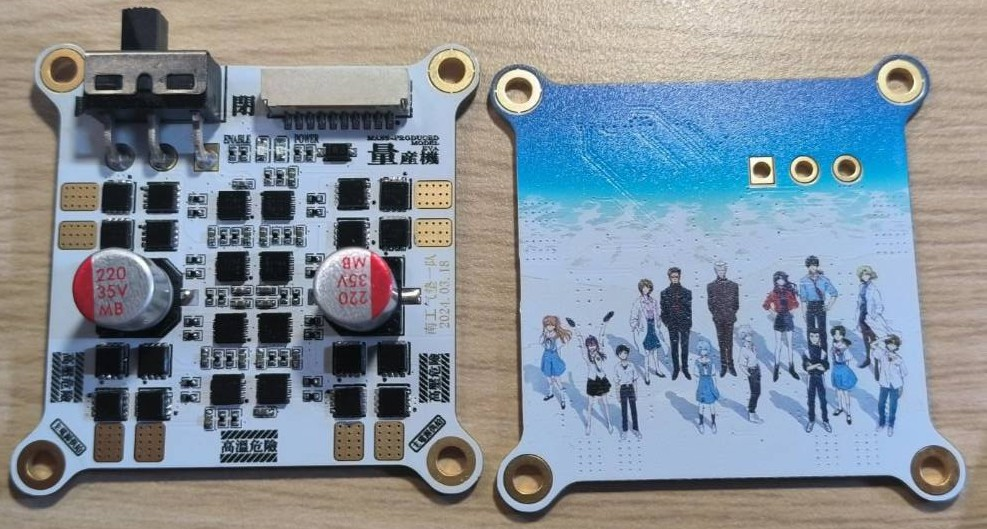
\includegraphics[scale=0.3]{./pic/chapter05/you-shua-qu-dong.jpg}
    \caption{有刷驱动 PCB}
    \label{you-shua}
    \end{figure}

\subsection{气垫船结构安装}
气垫船船体采用高强度PLA材料3D打印成型，通过优化填充结构实现轻量化设计；模块化分为主浮体舱、动力舱与操控舱，使用定位销与M3螺钉装配，接缝处进行密封处理；关键受力部位嵌入螺纹金属件增强连接强度。船体表面经打磨后喷涂环氧底漆与聚氨酯面漆，形成防水涂层。柔性裙边通过卡扣与船体连接，底部设有规则泄流孔以均衡气垫压力，如图\ref{fig:four_images}所示。
\begin{figure}[h]
    \centering
    % 第一行
    \subfigure[系统前视图]{
        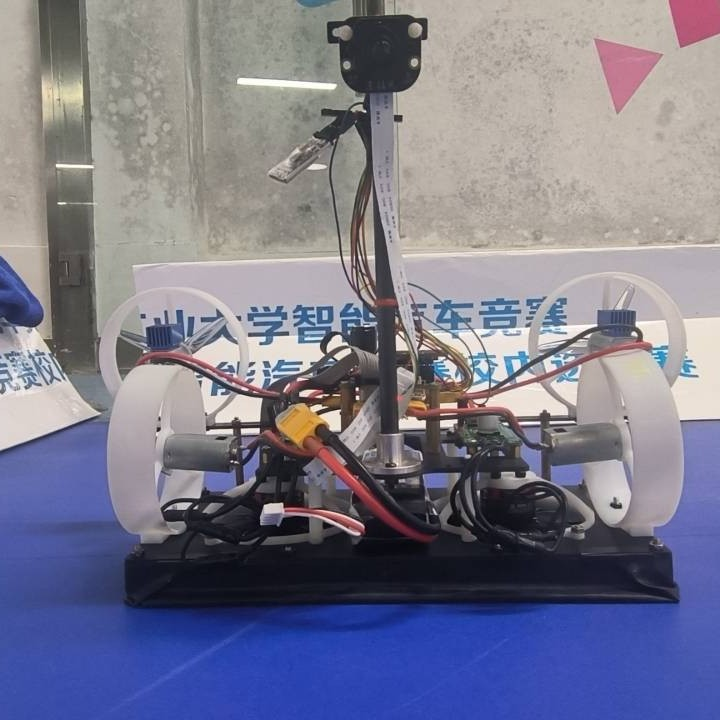
\includegraphics[scale=0.24]{./pic/chapter05/xi-tong-qian.jpg}
        \label{fig:sub1}
    }
    \quad
    \subfigure[系统后视图]{
        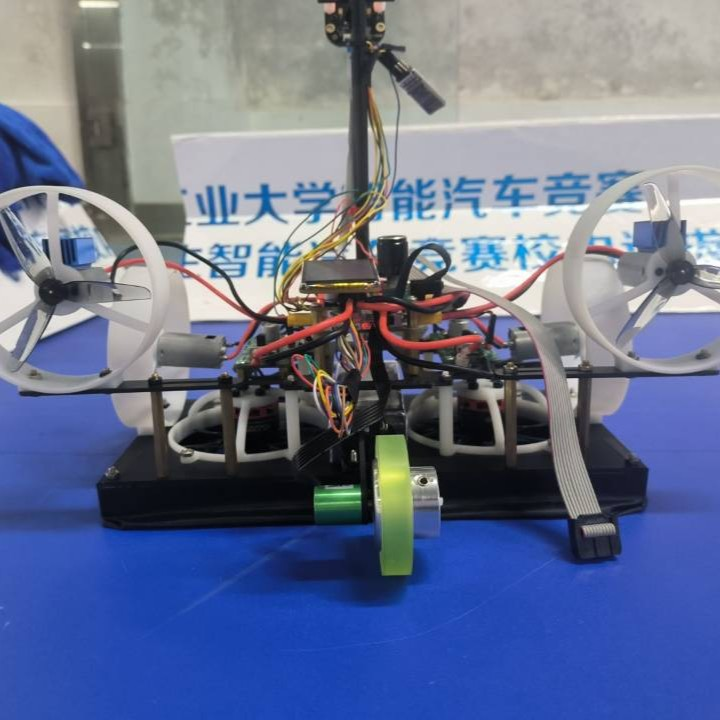
\includegraphics[scale=0.24]{./pic/chapter05/xi-tong-hou.jpg}
        \label{fig:sub2}
    }
    
    % 第二行
    \subfigure[系统侧视图]{
        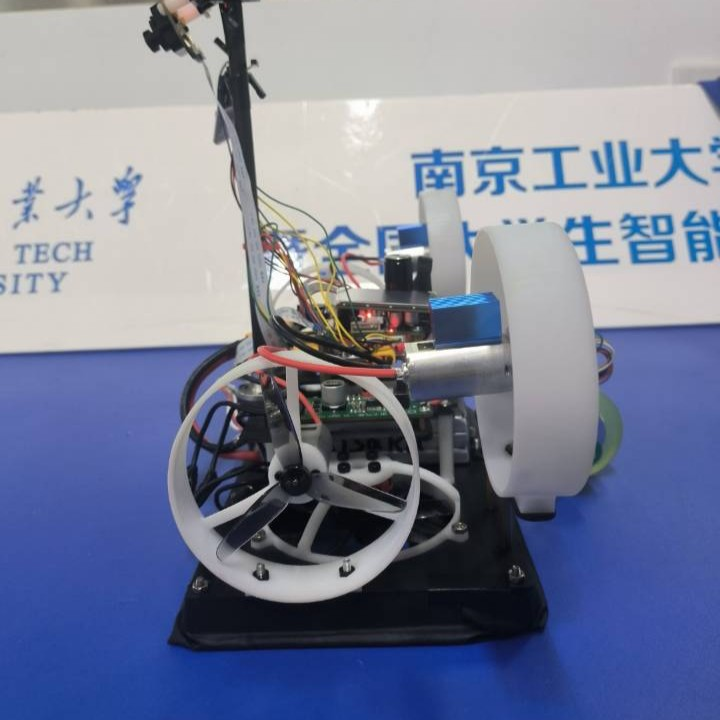
\includegraphics[scale=0.24]{./pic/chapter05/xi-tong-ce.jpg}
        \label{fig:sub3}
    }
    \quad
    \subfigure[系统上视图]{
        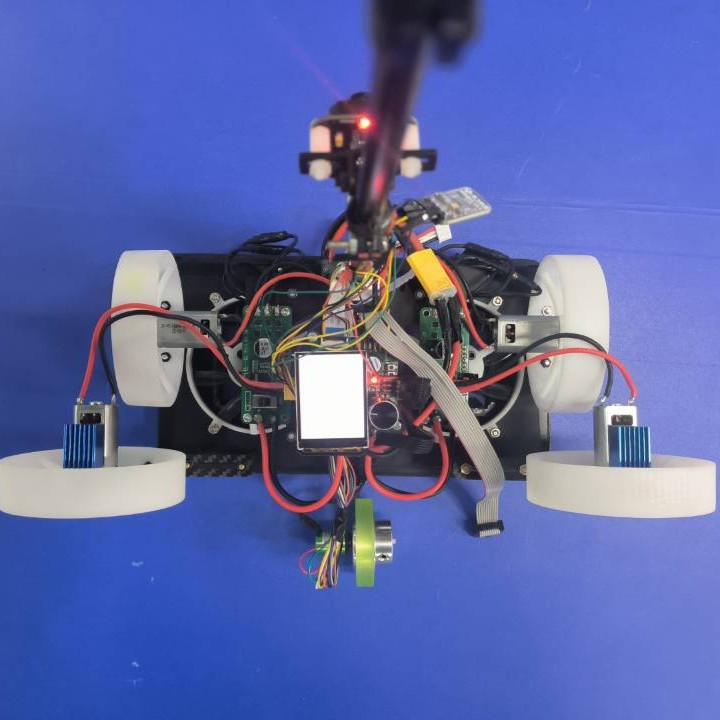
\includegraphics[scale=0.24]{./pic/chapter05/xi-tong-shang.jpg}
        \label{fig:sub4}
    }
    \caption{气垫船系统多视角图}
    \label{fig:four_images}
\end{figure}

% \begin{table}[htbp]
%     \centering
%     \caption{气垫船主要部件安装参数}
%     \label{tab:components-installation}
%     \begin{tabular}{lccc}
%         \toprule
%         \textbf{部件名称} & \textbf{安装位置} & \textbf{固定方式} & \textbf{连接线规格} \\
%         \midrule
%         主推进电机 & 船尾中心 & M3螺丝×4 & AWG18硅胶线 \\
%         升降风扇 & 船体中部 & M2.5螺丝×3 & AWG20硅胶线 \\
%         电源模块 & 重心位置 & 双面胶+扎带 & AWG14电源线 \\
%         传感器模块 & 船首 & 3M胶贴 & FPC排线 \\
%         \bottomrule
%     \end{tabular}
% \end{table}

% \subsubsection{电气系统安装}
% \label{subsec:electrical-installation}

% \begin{enumerate}
%     \item \textbf{动力系统接线}：
%     \begin{itemize}
%         \item 使用XT60接口连接锂电池（3S 2200mAh）
%         \item 30A电调与CH32的PWM输出引脚连接
%         \item 电机三相线按U/V/W顺序连接
%     \end{itemize}
    
%     \item \textbf{传感器系统接线}：
%     \begin{itemize}
%         \item MPU6050六轴传感器通过I2C接口连接（SDA-PB7，SCL-PB6）
%         \item GPS模块通过UART连接（TX-PA10，RX-PA9）
%         \item 超声波测距模块连接至ADC引脚（PA1）
%     \end{itemize}
    
%     \item \textbf{线束整理}：
%     \begin{itemize}
%         \item 使用尼龙编织网包裹线束
%         \item 电源线与信号线分离布线
%         \item 关键连接点采用热缩管保护
%     \end{itemize}
% \end{enumerate}

% \subsection{功能模块调试}
% \label{sec:module-debugging}

% \subsubsection{CH32核心模块调试}
% \label{subsec:ch32-debug}

% \textbf{调试工具配置}：
% \begin{verbatim}
% 开发环境：Keil MDK v5.30
% 调试器：ST-Link V2
% 串口工具：Tera Term 4.106
% \end{verbatim}

% \textbf{调试步骤}：
% \begin{enumerate}
%     \item \textbf{最小系统测试}：
%     \begin{itemize}
%         \item 上电测试3.3V电源输出（误差±0.05V）
%         \item 测量8MHz晶振起振波形（峰峰值≥800mV）
%         \item 测试复位电路功能
%     \end{itemize}
    
%     \item \textbf{固件下载测试}：
%     \begin{itemize}
%         \item 通过SWD接口下载测试程序
%         \item 验证Flash编程功能
%         \item 测试RAM读写正确性
%     \end{itemize}
    
%     \item \textbf{外设功能测试}：
%     \begin{itemize}
%         \item GPIO控制LED闪烁测试（频率1Hz）
%         \item PWM输出测试（频率50Hz，占空比0-100\%可调）
%         \item ADC采样测试（12位分辨率，误差<±2LSB）
%         \item UART通信测试（波特率115200，误码率<0.001\%）
%     \end{itemize}
% \end{enumerate}

% \subsubsection{动力系统调试}
% \label{subsec:power-debug}


% \textbf{电机调试参数设置}：
% \begin{equation}
%     PWM_{duty} = K_p \times (V_{target} - V_{current}) + K_i \times \int (V_{target} - V_{current}) dt
% \end{equation}


% \subsubsection{传感器模块调试}
% \label{subsec:sensor-debug}

% \textbf{调试结果记录}：
% \begin{table}[htbp]
%     \centering
%     \caption{传感器校准数据}
%     \label{tab:sensor-calibration}
%     \begin{tabular}{lcccc}
%         \toprule
%         \textbf{传感器} & \textbf{测量范围} & \textbf{分辨率} & \textbf{误差} & \textbf{校准后误差} \\
%         \midrule
%         MPU6050加速度计 & ±4g & 0.0012g & 0.05g & 0.01g \\
%         MPU6050陀螺仪 & ±500°/s & 0.015°/s & 1.5°/s & 0.3°/s \\
%         GPS模块 & - & 2.5m & 5m & 2.5m \\
%         超声波传感器 & 2-400cm & 0.3cm & ±1cm & ±0.5cm \\
%         \bottomrule
%     \end{tabular}
% \end{table}

% \subsubsection{IMU传感器校准}
% \label{subsubsec:imu-calibration}

% \textbf{六点校准法步骤}：
% \begin{enumerate}
%     \item 将气垫船水平放置，记录加速度计零点偏移
%     \item 分别绕X、Y、Z轴旋转±90°，采集陀螺仪数据
%     \item 使用最小二乘法计算校准矩阵：
%     \begin{equation}
%         \begin{bmatrix}
%             a_x' \\ a_y' \\ a_z'
%         \end{bmatrix}
%         =
%         \begin{bmatrix}
%             S_x & 0 & 0 \\
%             0 & S_y & 0 \\
%             0 & 0 & S_z
%         \end{bmatrix}
%         \begin{bmatrix}
%             a_x - O_x \\ a_y - O_y \\ a_z - O_z
%         \end{bmatrix}
%     \end{equation}
%     \item 将校准参数保存至CH32的Flash中
% \end{enumerate}

% \subsubsection{GPS定位调试}
% \label{subsubsec:gps-debug}

% \textbf{NMEA数据解析测试}：
% \begin{itemize}
%     \item 测试GGA语句解析（经纬度、海拔、卫星数）
%     \item 测试RMC语句解析（速度、航向、时间）
%     \item 测试定位精度：静态<2.5m，动态<5m
% \end{itemize}

% \subsection{系统整体调试}
% \label{sec:system-integration}

% \subsubsection{控制算法联调}
% \label{subsec:control-algorithm}

% \subsubsection{通信系统测试}
% \label{subsec:communication-test}

% \textbf{无线通信测试配置}：
% \begin{table}[htbp]
%     \centering
%     \caption{无线通信性能测试}
%     \label{tab:wireless-test}
%     \begin{tabular}{lcccc}
%         \toprule
%         \textbf{测试项目} & \textbf{距离(m)} & \textbf{丢包率(\%)} & \textbf{延迟(ms)} & \textbf{结果} \\
%         \midrule
%         视距通信 & 10 & 0.1 & 12 & 合格 \\
%         视距通信 & 50 & 0.5 & 15 & 合格 \\
%         有障碍物 & 30 & 2.3 & 25 & 基本合格 \\
%         运动状态 & 20 & 1.8 & 18 & 合格 \\
%         \bottomrule
%     \end{tabular}
% \end{table}

% \subsubsection{实船水上测试}
% \label{subsec:water-test}

% \textbf{测试环境}：
% \begin{itemize}
%     \item 测试场地：室内游泳池，水面20m×10m
%     \item 水深：1.5m
%     \item 环境温度：25°C
%     \item 风速：<1m/s（室内无风）
% \end{itemize}

% \textbf{性能测试结果}：
% \begin{enumerate}
%     \item \textbf{起浮测试}：从静止到完全起浮时间2.8秒
%     \item \textbf{高度保持}：目标高度10cm，实际高度波动±1.5cm
%     \item \textbf{转向测试}：最小转弯半径1.2m
%     \item \textbf{续航测试}：满载续航时间18分钟
%     \item \textbf{抗干扰测试}：人为制造波浪（高3cm），系统恢复时间2秒
% \end{enumerate}

% \subsection{本章小结}
% \label{sec:installation-summary}

% 本章完成了基于CH32微控制器的气垫船控制系统安装调试工作，主要包括：

% \begin{enumerate}
%     \item \textbf{硬件安装方面}：完成了CH32最小系统、气垫船结构和电气系统的安装，确保机械结构稳固，电气连接可靠
    
%     \item \textbf{模块调试方面}：
%     \begin{itemize}
%         \item CH32核心模块功能正常，所有外设工作稳定
%         \item 动力系统响应迅速，PWM控制精度满足要求
%         \item 传感器模块经过校准后精度显著提高
%     \end{itemize}
    
%     \item \textbf{系统联调方面}：
%     \begin{itemize}
%         \item 控制算法实现预定功能，气垫船姿态稳定
%         \item 通信系统在50米范围内性能可靠
%         \item 实船测试验证了系统设计的正确性
%     \end{itemize}
% \end{enumerate}

% 调试过程中发现并解决了以下主要问题：
% \begin{itemize}
%     \item 电机启动时需要最小30\%占空比才能克服静摩擦
%     \item IMU传感器受电机振动影响，增加了软件滤波算法
%     \item 无线通信在障碍物环境中性能下降，优化了通信协议
% \end{itemize}

% 经过系统安装调试，基于CH32的气垫船控制系统达到设计要求，为后续的功能测试和实际应用奠定了基础。所有调试数据和参数已记录存档，为系统维护和升级提供依据。